% (C) Brett Klamer - MIT - http://opensource.org/licenses/MIT
% Please contact me if you find any errors or make improvements
% Contact details at brettklamer.com

\documentclass[11pt,letterpaper,english,oneside]{article}\usepackage[]{graphicx}\usepackage[]{xcolor}
% maxwidth is the original width if it is less than linewidth
% otherwise use linewidth (to make sure the graphics do not exceed the margin)
\makeatletter
\def\maxwidth{ %
  \ifdim\Gin@nat@width>\linewidth
    \linewidth
  \else
    \Gin@nat@width
  \fi
}
\makeatother

\definecolor{fgcolor}{rgb}{0.345, 0.345, 0.345}
\newcommand{\hlnum}[1]{\textcolor[rgb]{0.686,0.059,0.569}{#1}}%
\newcommand{\hlstr}[1]{\textcolor[rgb]{0.192,0.494,0.8}{#1}}%
\newcommand{\hlcom}[1]{\textcolor[rgb]{0.678,0.584,0.686}{\textit{#1}}}%
\newcommand{\hlopt}[1]{\textcolor[rgb]{0,0,0}{#1}}%
\newcommand{\hlstd}[1]{\textcolor[rgb]{0.345,0.345,0.345}{#1}}%
\newcommand{\hlkwa}[1]{\textcolor[rgb]{0.161,0.373,0.58}{\textbf{#1}}}%
\newcommand{\hlkwb}[1]{\textcolor[rgb]{0.69,0.353,0.396}{#1}}%
\newcommand{\hlkwc}[1]{\textcolor[rgb]{0.333,0.667,0.333}{#1}}%
\newcommand{\hlkwd}[1]{\textcolor[rgb]{0.737,0.353,0.396}{\textbf{#1}}}%
\let\hlipl\hlkwb

\usepackage{framed}
\makeatletter
\newenvironment{kframe}{%
 \def\at@end@of@kframe{}%
 \ifinner\ifhmode%
  \def\at@end@of@kframe{\end{minipage}}%
  \begin{minipage}{\columnwidth}%
 \fi\fi%
 \def\FrameCommand##1{\hskip\@totalleftmargin \hskip-\fboxsep
 \colorbox{shadecolor}{##1}\hskip-\fboxsep
     % There is no \\@totalrightmargin, so:
     \hskip-\linewidth \hskip-\@totalleftmargin \hskip\columnwidth}%
 \MakeFramed {\advance\hsize-\width
   \@totalleftmargin\z@ \linewidth\hsize
   \@setminipage}}%
 {\par\unskip\endMakeFramed%
 \at@end@of@kframe}
\makeatother

\definecolor{shadecolor}{rgb}{.97, .97, .97}
\definecolor{messagecolor}{rgb}{0, 0, 0}
\definecolor{warningcolor}{rgb}{1, 0, 1}
\definecolor{errorcolor}{rgb}{1, 0, 0}
\newenvironment{knitrout}{}{} % an empty environment to be redefined in TeX

\usepackage{alltt} % article class is a standard class
%==============================================================================
%Load Packages
%==============================================================================
\usepackage[left=1in,right=1in,top=1in,bottom=1in]{geometry} % easy page margins
\usepackage[utf8]{inputenc} % editor uses utf-8 encoding
\usepackage[T1]{fontenc} % T1 font pdf output
\usepackage{lmodern} % Latin modern roman font
\usepackage{bm, bbm} % bold and blackboard bold math symbols
\usepackage{amsmath, amsfonts, amssymb, amsthm} % math packages
\usepackage[final]{microtype} % better microtypography
\usepackage{graphicx} % for easier grahics handling
\usepackage[hidelinks, colorlinks=true, linkcolor = blue, urlcolor = blue]{hyperref} % to create hyperlinks
\usepackage{float} % tells floats to stay [H]ere!
\usepackage{mdframed} % it's better than framed. knitr uses framed so settings won't conflict
\usepackage{enumitem} % nice lists
\usepackage{fancyhdr} % nice headers
\usepackage{caption}  % to control figure and table captions

\captionsetup{width=0.9\textwidth, justification = raggedright}

%==============================================================================
% Enter name and homework title here
%==============================================================================
\author{Eugene Katsevich}
\title{Creating high quality figures}


%==============================================================================
% Put title and author in PDF properties
%==============================================================================
\makeatletter % change interpretation of @
\hypersetup{pdftitle={\@title},pdfauthor={\@author}}


%==============================================================================
% Header settings
%==============================================================================
\pagestyle{fancy} % turns on fancy header styles
\fancyhf{} % clear all header and footer fields
\makeatletter
\lhead{\@author} % left header
\chead{\@title} % center header
\makeatother
\rhead{Page \thepage} % right header
\setlength{\headheight}{13.6pt} % fixes minor warning
\makeatother % change back interpretation of @

%==============================================================================
% List spacing
%==============================================================================
\setlist[itemize]{parsep=0em} % fix itemize spacing
\setlist[enumerate]{parsep=0em} % fix enumerate spacing

%==============================================================================
% set knitr options
%==============================================================================
% latex (change space before and after knitr kframe; based on framed package)
\setlength{\OuterFrameSep}{0.3em}
% R


\IfFileExists{upquote.sty}{\usepackage{upquote}}{}
\begin{document}

\maketitle

This document gives some suggestions on how to create high-quality figures, an essential skill for communicating your results effectively, whether in a paper, talk, or poster. Some of the material is drawn from \href{https://r4ds.had.co.nz/graphics-for-communication.html}{Chapter 28} of R for Data Science. 

\section{Sizing}

Once you have created a plot in R, you need to export it to include it in your paper, talk, or poster. For example, suppose we have the plot \verb|p| defined as below:
\begin{knitrout}
\definecolor{shadecolor}{rgb}{0.969, 0.969, 0.969}\color{fgcolor}\begin{kframe}
\begin{alltt}
\hlstd{test_data} \hlkwb{<-} \hlkwd{tibble}\hlstd{(}\hlkwc{x} \hlstd{=} \hlkwd{rnorm}\hlstd{(}\hlnum{10}\hlstd{),} \hlkwc{y} \hlstd{=} \hlkwd{rnorm}\hlstd{(}\hlnum{10}\hlstd{))}
\hlstd{p} \hlkwb{<-} \hlstd{test_data} \hlopt \hlkwd{ggplot}\hlstd{(}\hlkwd{aes}\hlstd{(}\hlkwc{x} \hlstd{= x,} \hlkwc{y} \hlstd{= y))} \hlopt{+} \hlkwd{geom_point}\hlstd{()} \hlopt{+} \hlkwd{theme_bw}\hlstd{()}
\end{alltt}
\end{kframe}
\end{knitrout}
\noindent You should save it as a PDF via \verb|ggsave|:
\begin{knitrout}
\definecolor{shadecolor}{rgb}{0.969, 0.969, 0.969}\color{fgcolor}\begin{kframe}
\begin{alltt}
\hlkwd{ggsave}(plot = p, 
       filename = \hlstr{"figures-and-tables/test_plot.pdf"}, 
       device = \hlstr{"pdf"}, 
       width = ???, 
       height = ???)
\end{alltt}
\end{kframe}
\end{knitrout}
\noindent Here, the question marks should be the width and height of the figure, in inches. Choose these to get a reasonable aspect ratio and a reasonable overall plot size. The aspect ratio (i.e. ratio of width to height) of your plots should be consistent with their content; e.g. box plots are usually relatively narrow, and scatter plots often make sense with equal aspect ratios. The overall plot size should be such that the smallest text in your plots should be roughly the same size as the text in the rest of your slides/paper/poster. Figures~\ref{fig:test-plot-small}, \ref{fig:test-plot-medium}, and~\ref{fig:test-plot-large} consider the width and length of the figure to be 1 inch, 2.5 inches, and 5 inches, respectively. The medium-sized plot (Figure~\ref{fig:test-plot-medium}) appears to be the most sensible choice. It usually takes a few tries to find an appropriate size for a figure. If the figures are going into a LaTeX report, I recommend \verb|\includegraphics| using the original scale of the figure you created (i.e. not using commands like \verb|width = 0.8\textwidth|): 
\begin{verbatim}
\begin{figure}[h!]
\centering
\includegraphics{figures-and-tables/test_plot.pdf}
\caption{A test plot.}
\label{fig:test-plot}
\end{figure}
\end{verbatim}
This will create consistent font sizes throughout your document.



\begin{figure}[h!]
\centering
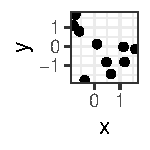
\includegraphics{figures-and-tables/test_plot_small.pdf}
\caption{The plot saved as 1in by 1in.}
\label{fig:test-plot-small}
\end{figure}

\begin{figure}[h!]
\centering
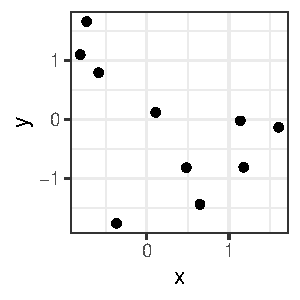
\includegraphics{figures-and-tables/test_plot_medium.pdf}
\caption{The plot saved as 2in by 2in.}
\label{fig:test-plot-medium}
\end{figure}

\begin{figure}[h!]
\centering
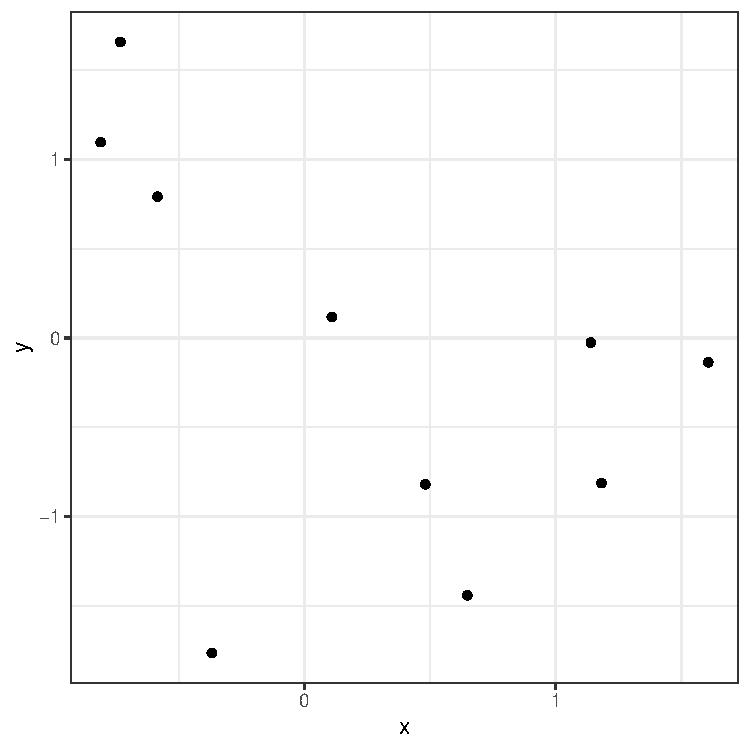
\includegraphics{figures-and-tables/test_plot_large.pdf}
\caption{The plot saved as 5in by 5in.}
\label{fig:test-plot-large}
\end{figure}


\section{Titles}

Each plot should include informative axis and legend titles. For example, consider the code below (drawn from R4DS Chapter 28), which produces the plot in Figure~\ref{fig:cars-unlabeled}.
\begin{knitrout}
\definecolor{shadecolor}{rgb}{0.969, 0.969, 0.969}\color{fgcolor}\begin{kframe}
\begin{alltt}
\hlcom{# a plot without clear axis and legend titles}
\hlstd{p} \hlkwb{<-} \hlstd{mpg} \hlopt
  \hlkwd{ggplot}\hlstd{(}\hlkwd{aes}\hlstd{(}\hlkwc{x} \hlstd{= displ,} \hlkwc{y} \hlstd{= hwy))} \hlopt{+}
  \hlkwd{geom_point}\hlstd{(}\hlkwd{aes}\hlstd{(}\hlkwc{color} \hlstd{= class))} \hlopt{+}
  \hlkwd{geom_smooth}\hlstd{(}\hlkwc{se} \hlstd{=} \hlnum{FALSE}\hlstd{)} \hlopt{+}
  \hlkwd{theme_bw}\hlstd{()}

\hlcom{# save plot}
\hlkwd{ggsave}\hlstd{(}\hlkwc{plot} \hlstd{= p,}
       \hlkwc{filename} \hlstd{=} \hlstr{"figures-and-tables/cars-unlabeled.pdf"}\hlstd{,}
       \hlkwc{device} \hlstd{=} \hlstr{"pdf"}\hlstd{,}
       \hlkwc{width} \hlstd{=} \hlnum{5}\hlstd{,}
       \hlkwc{height} \hlstd{=} \hlnum{3.75}\hlstd{)}
\end{alltt}
\end{kframe}
\end{knitrout}
This is a plot of fuel efficiency versus engine displacement for various types of cars, but the axis and legend labels on the plot do not make this very clear. 
\begin{figure}[h!]
\centering
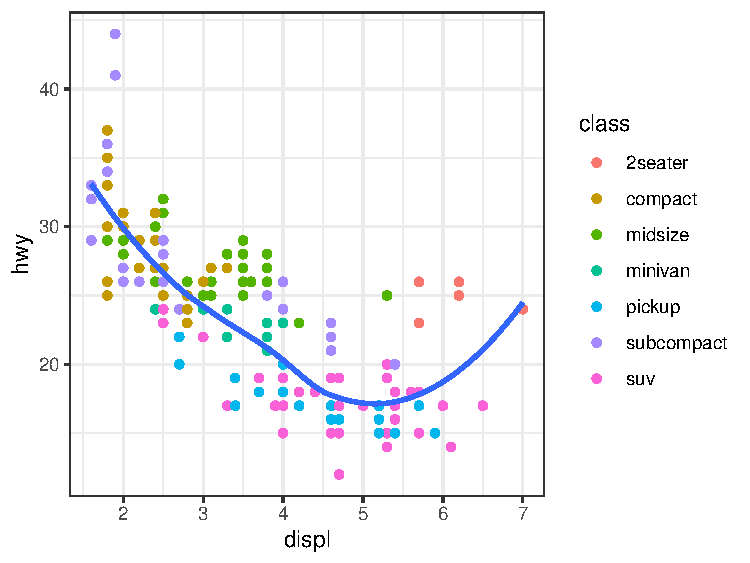
\includegraphics{figures-and-tables/cars-unlabeled.pdf}
\caption{A plot without clear titles.}
\label{fig:cars-unlabeled}
\end{figure}
We can easily add informative titles to this plot using \texttt{labs}, resulting in Figure~\ref{fig:cars-labeled}, which is much easier to understand. 
\begin{knitrout}
\definecolor{shadecolor}{rgb}{0.969, 0.969, 0.969}\color{fgcolor}\begin{kframe}
\begin{alltt}
\hlcom{# a plot with clear axis and legend titles}
\hlstd{p} \hlkwb{<-} \hlstd{mpg} \hlopt
  \hlkwd{ggplot}\hlstd{(}\hlkwd{aes}\hlstd{(}\hlkwc{x} \hlstd{= displ,} \hlkwc{y} \hlstd{= hwy))} \hlopt{+}
  \hlkwd{geom_point}\hlstd{(}\hlkwd{aes}\hlstd{(}\hlkwc{color} \hlstd{= class))} \hlopt{+}
  \hlkwd{geom_smooth}\hlstd{(}\hlkwc{se} \hlstd{=} \hlnum{FALSE}\hlstd{)} \hlopt{+}
  \hlkwd{labs}\hlstd{(}
    \hlkwc{x} \hlstd{=} \hlstr{"Engine displacement (liters)"}\hlstd{,}
    \hlkwc{y} \hlstd{=} \hlstr{"Highway fuel economy (miles per gallon)"}\hlstd{,}
    \hlkwc{colour} \hlstd{=} \hlstr{"Car type"}
  \hlstd{)} \hlopt{+}
  \hlkwd{theme_bw}\hlstd{()}

\hlcom{# save plot}
\hlkwd{ggsave}\hlstd{(}\hlkwc{plot} \hlstd{= p,}
       \hlkwc{filename} \hlstd{=} \hlstr{"figures-and-tables/cars-labeled.pdf"}\hlstd{,}
       \hlkwc{device} \hlstd{=} \hlstr{"pdf"}\hlstd{,}
       \hlkwc{width} \hlstd{=} \hlnum{5}\hlstd{,}
       \hlkwc{height} \hlstd{=} \hlnum{3.75}\hlstd{)}
\end{alltt}
\end{kframe}
\end{knitrout}
\begin{figure}[h!]
\centering
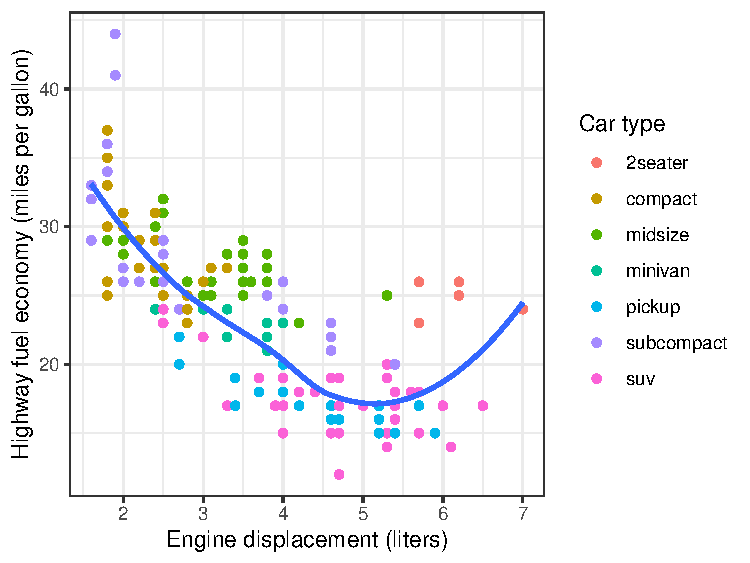
\includegraphics{figures-and-tables/cars-labeled.pdf}
\caption{(A plot with clear axis and legend titles). Fuel efficiency generally decreases with engine size; two-seaters (sports cars) are an exception because of their light weight.}
\label{fig:cars-labeled}
\end{figure}
\noindent Plots might or might not need overall titles; often the axis titles speak for themselves and the message of the plot can be conveyed in the caption (as in Figure~\ref{fig:cars-labeled}.) To add plot titles if necessary, use the \verb|title| argument to \verb|labs()|.

If applicable, axis titles should also include the units of measurement, e.g. liters or miles per gallon as in Figure~\ref{fig:cars-labeled}. If axis titles involve mathematical formulas, these should be typeset appropriately. The code below (drawn from R4DS Chapter 28) and Figure~\ref{fig:formulas}, which it produces, illustrate how to do this. More examples can be found at \href{https://rdrr.io/r/grDevices/plotmath.html}{\texttt{?plotmath}}.
\begin{knitrout}
\definecolor{shadecolor}{rgb}{0.969, 0.969, 0.969}\color{fgcolor}\begin{kframe}
\begin{alltt}
\hlcom{# a plot illustrating how to include formulas in axis titles}
\hlstd{p} \hlkwb{=} \hlkwd{tibble}\hlstd{(}\hlkwc{x} \hlstd{=} \hlkwd{runif}\hlstd{(}\hlnum{10}\hlstd{),}
       \hlkwc{y} \hlstd{=} \hlkwd{runif}\hlstd{(}\hlnum{10}\hlstd{))} \hlopt
  \hlkwd{ggplot}\hlstd{(}\hlkwd{aes}\hlstd{(x, y))} \hlopt{+}
  \hlkwd{geom_point}\hlstd{()} \hlopt{+}
  \hlkwd{labs}\hlstd{(}\hlkwc{x} \hlstd{=} \hlkwd{quote}\hlstd{(}\hlkwd{sum}\hlstd{(x[i]} \hlopt{^} \hlnum{2}\hlstd{, i} \hlopt{==} \hlnum{1}\hlstd{, n)),}
       \hlkwc{y} \hlstd{=} \hlkwd{quote}\hlstd{(alpha} \hlopt{+} \hlstd{beta} \hlopt{+} \hlkwd{frac}\hlstd{(delta, theta)))} \hlopt{+}
  \hlkwd{theme_bw}\hlstd{()}

\hlcom{# save the plot}
\hlkwd{ggsave}\hlstd{(}\hlkwc{plot} \hlstd{= p,}
       \hlkwc{filename} \hlstd{=} \hlstr{"figures-and-tables/fig-formulas.pdf"}\hlstd{,}
       \hlkwc{device} \hlstd{=} \hlstr{"pdf"}\hlstd{,}
       \hlkwc{width} \hlstd{=} \hlnum{2.5}\hlstd{,}
       \hlkwc{height} \hlstd{=} \hlnum{2.5}\hlstd{)}
\end{alltt}
\end{kframe}
\end{knitrout}
\begin{figure}[h!]
\centering
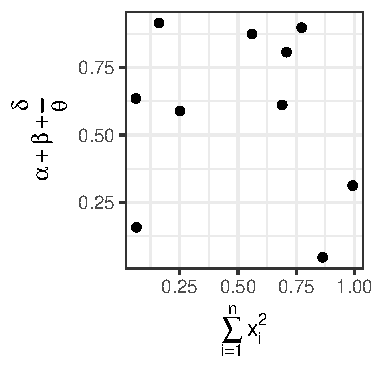
\includegraphics{figures-and-tables/fig-formulas.pdf}
\caption{An illustration of using formulas in axis titles.}
\label{fig:formulas}
\end{figure}

\section{Captions}

Figures should have informative captions to help readers understand what information is displayed and how to interpret it. 

\section{Layout}

Sometimes, two or more plots make sense to present together in a single figure. This can be accomplished in two ways. If the different plots convey the same type of information but for different slices of the data, then \verb|facet_grid| and \verb|facet_wrap| are the best way of laying out these plots. For example, the code below and Figure~\ref{fig:facet-wrap} illustrates \verb|facet_wrap| for the \texttt{mpg} data used in Figures~\ref{fig:cars-unlabeled} and~\ref{fig:cars-labeled}.

\begin{knitrout}
\definecolor{shadecolor}{rgb}{0.969, 0.969, 0.969}\color{fgcolor}\begin{kframe}
\begin{alltt}
\hlcom{# illustrate how to use facet_wrap to create a multi-panel plot}
\hlstd{p} \hlkwb{=} \hlstd{mpg} \hlopt
  \hlkwd{filter}\hlstd{(class} \hlopt
           \hlkwd{c}\hlstd{(}\hlstr{"2seater"}\hlstd{,} \hlstr{"compact"}\hlstd{,} \hlstr{"midsize"}\hlstd{))} \hlopt  \hlcom{# select 3 classes of cars}
  \hlkwd{ggplot}\hlstd{(}\hlkwd{aes}\hlstd{(}\hlkwc{x} \hlstd{= displ,} \hlkwc{y} \hlstd{= hwy))} \hlopt{+}
  \hlkwd{geom_point}\hlstd{()} \hlopt{+}
  \hlkwd{facet_wrap}\hlstd{(class} \hlopt{~} \hlstd{.)} \hlopt{+}                           \hlcom{# separate panels per class}
  \hlkwd{labs}\hlstd{(}
    \hlkwc{x} \hlstd{=} \hlstr{"Engine displacement (liters)"}\hlstd{,}
    \hlkwc{y} \hlstd{=} \hlstr{"Highway fuel economy\textbackslash{}n(miles per gallon)"}\hlstd{,} \hlcom{# line break in axis title}
  \hlstd{)} \hlopt{+}
  \hlkwd{theme_bw}\hlstd{()}

\hlcom{# save the plot}
\hlkwd{ggsave}\hlstd{(}\hlkwc{plot} \hlstd{= p,}
       \hlkwc{filename} \hlstd{=} \hlstr{"figures-and-tables/facet-wrap.pdf"}\hlstd{,}
       \hlkwc{device} \hlstd{=} \hlstr{"pdf"}\hlstd{,}
       \hlkwc{width} \hlstd{=} \hlnum{5.5}\hlstd{,}
       \hlkwc{height} \hlstd{=} \hlnum{2.25}\hlstd{)}
\end{alltt}
\end{kframe}
\end{knitrout}
\begin{figure}[h!]
\centering
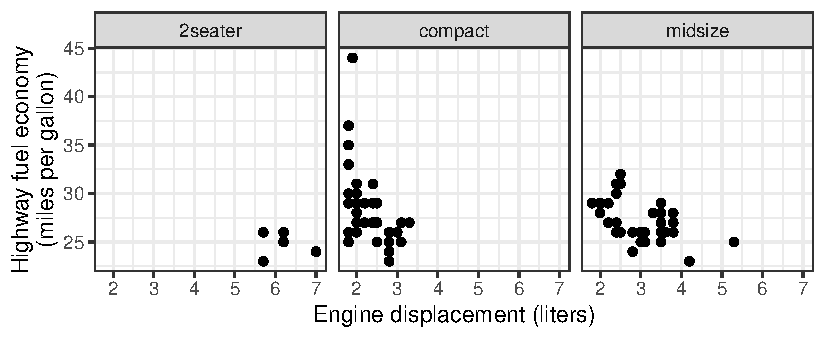
\includegraphics{figures-and-tables/facet-wrap.pdf}
\caption{An illustration of using \texttt{facet\_wrap} to create a multi-panel plot.}
\label{fig:facet-wrap}
\end{figure}

If the plots convey different types of information, then they should be created separately and then concatenated together using \verb|plot_grid| from the \verb|cowplot| package. An example is shown below and in Figure~\ref{fig:cowplot-demo}. Note that the figure caption should reference the subpanels by their labels (in this case, a and b).
\begin{knitrout}
\definecolor{shadecolor}{rgb}{0.969, 0.969, 0.969}\color{fgcolor}\begin{kframe}
\begin{alltt}
\hlcom{# illustration of using cowplot to concatenate multiple plots}
\hlkwd{library}\hlstd{(cowplot)}

\hlcom{# first plot: box plot of fuel economy by car type}
\hlstd{p1} \hlkwb{=} \hlstd{mpg} \hlopt
  \hlkwd{mutate}\hlstd{(}\hlkwc{class} \hlstd{=}                         \hlcom{# re-order car classes by fuel economy}
           \hlkwd{fct_reorder}\hlstd{(class, hwy))} \hlopt
  \hlkwd{ggplot}\hlstd{(}\hlkwd{aes}\hlstd{(}\hlkwc{x} \hlstd{= class,} \hlkwc{y} \hlstd{= hwy,} \hlkwc{fill} \hlstd{= class))} \hlopt{+}
  \hlkwd{geom_boxplot}\hlstd{()} \hlopt{+}
  \hlkwd{labs}\hlstd{(}
    \hlkwc{x} \hlstd{=} \hlstr{"Car type"}\hlstd{,}
    \hlkwc{y} \hlstd{=} \hlstr{"Highway fuel economy\textbackslash{}n(miles per gallon)"}
  \hlstd{)} \hlopt{+}
  \hlkwd{theme_bw}\hlstd{()} \hlopt{+}
  \hlkwd{theme}\hlstd{(}\hlkwc{legend.position} \hlstd{=} \hlstr{"none"}\hlstd{,}        \hlcom{# remove legend and x axis text because }
        \hlkwc{axis.text.x} \hlstd{=} \hlkwd{element_blank}\hlstd{())}   \hlcom{#  information present in second plot}

\hlcom{# second plot: scatter plot of fuel economy versus car type}
\hlstd{p2} \hlkwb{=} \hlstd{mpg} \hlopt
  \hlkwd{mutate}\hlstd{(}\hlkwc{class} \hlstd{=}                         \hlcom{# re-order car classes by fuel economy}
           \hlkwd{fct_reorder}\hlstd{(class, hwy))} \hlopt
  \hlkwd{ggplot}\hlstd{(}\hlkwd{aes}\hlstd{(}\hlkwc{x} \hlstd{= displ,} \hlkwc{y} \hlstd{= hwy))} \hlopt{+}
  \hlkwd{geom_point}\hlstd{(}\hlkwd{aes}\hlstd{(}\hlkwc{color} \hlstd{= class))} \hlopt{+}
  \hlkwd{geom_smooth}\hlstd{(}\hlkwc{se} \hlstd{=} \hlnum{FALSE}\hlstd{)} \hlopt{+}
  \hlkwd{labs}\hlstd{(}
    \hlkwc{x} \hlstd{=} \hlstr{"Engine displacement (liters)"}\hlstd{,}
    \hlkwc{colour} \hlstd{=} \hlstr{"Car type"}
  \hlstd{)} \hlopt{+}
  \hlkwd{theme_bw}\hlstd{()} \hlopt{+}
  \hlkwd{theme}\hlstd{(}\hlkwc{axis.title.y} \hlstd{=} \hlkwd{element_blank}\hlstd{())}  \hlcom{# remove y axis title because already}
                                         \hlcom{#  present in the first plot}

\hlcom{# use plot_grid from cowplot to concatenate the two plots}
\hlstd{p} \hlkwb{=} \hlkwd{plot_grid}\hlstd{(p1,}
              \hlstd{p2,}
              \hlkwc{labels} \hlstd{=} \hlstr{"auto"}\hlstd{,}     \hlcom{# generate labels for subplots}
              \hlkwc{rel_widths} \hlstd{=} \hlkwd{c}\hlstd{(}\hlnum{1}\hlstd{,}\hlnum{2}\hlstd{),} \hlcom{# specify relative widths}
              \hlkwc{align} \hlstd{=} \hlstr{"h"}\hlstd{)}         \hlcom{# how to align subplots}

\hlcom{# save the plot}
\hlkwd{ggsave}\hlstd{(}\hlkwc{plot} \hlstd{= p,}
       \hlkwc{filename} \hlstd{=} \hlstr{"figures-and-tables/cowplot-demo.pdf"}\hlstd{,}
       \hlkwc{device} \hlstd{=} \hlstr{"pdf"}\hlstd{,}
       \hlkwc{width} \hlstd{=} \hlnum{5}\hlstd{,}
       \hlkwc{height} \hlstd{=} \hlnum{2.5}\hlstd{)}
\end{alltt}
\end{kframe}
\end{knitrout}
\begin{figure}[!htb]
\centering
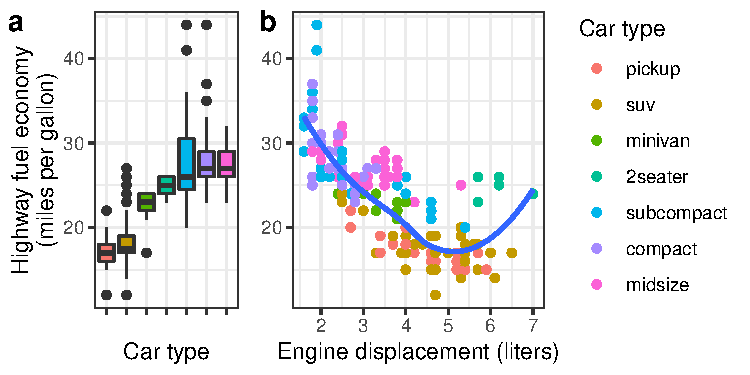
\includegraphics{figures-and-tables/cowplot-demo.pdf}
\caption{(An illustration of using \texttt{cowplot} to create a multi-panel plot.) Relationships between highway fuel economy and car type (a) and engine displacement (b). }
\label{fig:cowplot-demo}
\end{figure}

\vspace{2in}

\section{Further resources}

\begin{itemize}
\item \href{https://r4ds.had.co.nz/graphics-for-communication.html}{Chapter 28} of R for Data Science 
\item \href{https://journals.plos.org/ploscompbiol/article?id=10.1371/journal.pcbi.1003833}{Ten Simple Rules for Better Figures} (PLOS Computational Biology, 2014)
\item \href{https://b.nanes.org/figures/}{How to Create Publication-Quality Figures} (by Benjamin Nanes)
\end{itemize}

\end{document}
